\chapter{Vermogen en blindvermogen}
\label{vermogen}

Bij een spoel loopt de stroom 90° achter op de spanning.\\
Een spoel heeft geen weerstand, daarom heeft de idiale spoel geen vermogen. Er is echter wel iets wat gebeurt wat er is impendantie. Het
vermogen wat ontstaat heeft blind vermogen. Dit wordt aangegeven met de letter Q. 

Bij een condensator loop de stroom 90° voor op de spanning.\\
Bij een condensator geld het zelfde als bij de spoel. Bij de condesator wordt ook gewerkt met blind vermogen, Q. Dit vermogen is integenstelling
tot de spoel negatief.

Bij een weerstand loopt de stroom in fase met de spanning.\\
Enkel een weerstand heeft vermogen, wat wordt aangegeven met de letter P.

\section{Vermogensdriehoek}
Om de gegevens van schakelingen te berekenen wordt gebruik gemaakt van de vermogensdriehoek.

\begin{center}

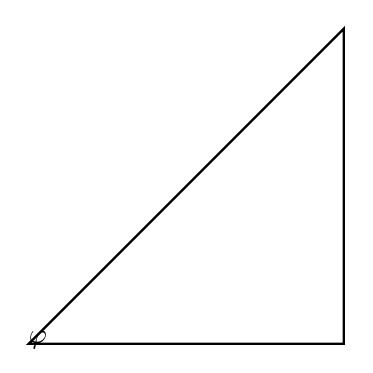
\begin{tikzpicture}[thick]
\coordinate (O) at (0,0);
\coordinate (A) at (4,0);
\coordinate (B) at (4,4);
\draw (O)--(A)--(B)--cycle;

\tkzLabelSegment[below=2pt](O,A){\textit{P}}
\tkzLabelSegment[left=2pt](O,B){\textit{S}}
\tkzLabelSegment[above right=2pt](A,B){\textit{Q}}

\tkzMarkAngle[fill= teal,size=0.8cm,%
opacity=.4](A,O,B)
\tkzLabelAngle[pos = 0.6](A,O,B){$\varphi $}

\end{tikzpicture}
\end{center}

binnen de driehoek geldt:\\
P= vermogen\\
Q= blind vermogen\\
S= schijnbaar vermogen\\

Hier is de formule voor het schijnbaar vermogen:
\begin{itemize}
    \item $S=\sqrt{P^2+Q^2}$
    \item $S= UI$
\end{itemize}

De formule voor het vermogen is:

$P= UI \cos \varphi=S \cos \varphi$

\vspace{5mm}

En de formule voor het blind vermogen is:

$Q= UI \sin \varphi=S \sin \varphi$

\vspace{5mm}

Doormiddel van de fromules:
\begin{itemize}
    \item $\cos \varphi =\frac{P}{S}$
    \item $\sin \varphi =\frac{Q}{S}$
    \item $\tan \varphi =\frac{Q}{P}$
\end{itemize}

kunnen met 2 waardes alle andere waardes worden berekend.

Daarnaast gelden de formules:

Spoel:

$X_L=\frac{Q_L}{I_L^2}$

$\omega L=\frac{Q_L}{I_L^2}$

$L=\frac{Q_L}{\omega I_L^2}$

\vspace{5mm}

of voor de spanning:

$X_L=\frac{Q_L}{U_L^2}$

$\omega L=\frac{Q_L}{U_L^2}$

$L=\frac{Q_L}{\omega U_L^2}$

\vspace{5mm}

Condensator:

$X_C=\frac{Q_C}{I_C^2}$

$\omega C=\frac{Q_C}{I_C^2}$

$C=\frac{I_C^2}{\omega Q_C}$

\vspace{5mm}

of voor de spanning:

$X_C=\frac{Q_C}{U_C^2}$

$\omega C=\frac{Q_C}{U_C^2}$

$C=\frac{U_C^2}{\omega Q_C}$

\vspace{5mm}

tot slot geld: 

$\theta = \theta _V - \theta _I$

\section{Impendantie driehoek}
Voor de impendantie is ook een driehoek te maken. Dit is de driehoek voor een spoel.

\begin{center}

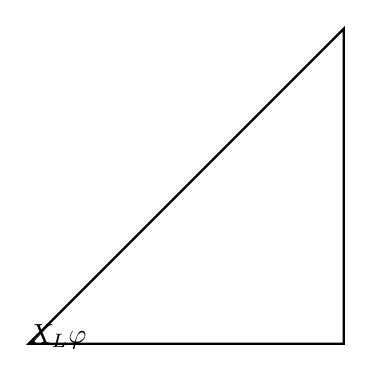
\begin{tikzpicture}[thick]
\coordinate (O) at (0,0);
\coordinate (A) at (4,0);
\coordinate (B) at (4,4);
\draw (O)--(A)--(B)--cycle;

\tkzLabelSegment[below=2pt](O,A){\textit{R}}
\tkzLabelSegment[left=2pt](O,B){\textit{Z}}
\tkzLabelSegment[above right=2pt](A,B){\textit{$X_L$}}

\tkzMarkAngle[fill= teal,size=0.8cm,%
opacity=.4](A,O,B)
\tkzLabelAngle[pos = 0.6](A,O,B){$\varphi $}

\end{tikzpicture}
\end{center}

Hier geldt:\\
R= weerstand\\
Z= impendantie\\
$X_L$= inductieve reactantie\\

De verschillen de waardes kunnen bepaald worden op de zelfde manier als bij de vermogensdriehoek.

\vspace{5mm}

Voor de Condensator geld het zelfde alleen is $X_L$ vervangen door $X_C$ en is de impendantie negatief.

\begin{center}

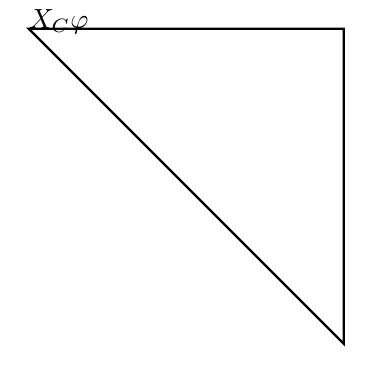
\begin{tikzpicture}[thick]
\coordinate (O) at (0,0);
\coordinate (A) at (4,0);
\coordinate (B) at (4,-4);
\draw (O)--(A)--(B)--cycle;

\tkzLabelSegment[above=2pt](O,A){\textit{R}}
\tkzLabelSegment[left=2pt](O,B){\textit{Z}}
\tkzLabelSegment[above right=2pt](A,B){\textit{$X_C$}}

\tkzMarkAngle[fill= teal,size=0.8cm,%
opacity=.4](B,O,A)
\tkzLabelAngle[pos = -0.6](A,O,B){$\varphi $}

\end{tikzpicture}
\end{center}

Meer informatie over de uitleg over vermogen en impendantie is te vinden in hoofdstuk 5.5 van het boek van Hambley 
\cite{leerboek}.